%
% File acl2017.tex
%
%% Based on the style files for ACL-2015, with some improvements
%%  taken from the NAACL-2016 style
%% Based on the style files for ACL-2014, which were, in turn,
%% based on ACL-2013, ACL-2012, ACL-2011, ACL-2010, ACL-IJCNLP-2009,
%% EACL-2009, IJCNLP-2008...
%% Based on the style files for EACL 2006 by 
%%e.agirre@ehu.es or Sergi.Balari@uab.es
%% and that of ACL 08 by Joakim Nivre and Noah Smith

\documentclass[11pt,a4paper]{article}
\usepackage[hyperref]{acl2017}
\usepackage{times}
\usepackage{latexsym}
\usepackage{xcolor}

\usepackage{url}

\aclfinalcopy % Uncomment this line for the final submission
%\def\aclpaperid{***} %  Enter the acl Paper ID here

%\setlength\titlebox{5cm}
% You can expand the titlebox if you need extra space
% to show all the authors. Please do not make the titlebox
% smaller than 5cm (the original size); we will check this
% in the camera-ready version and ask you to change it back.

% added
\usepackage{graphicx}
\usepackage{amsmath}
\usepackage{dsfont} %to have \mathds{1}

\newcommand\BibTeX{B{\sc ib}\TeX}

\title{Identification and quantification of colours in children's drawings}

\author{Christelle Cocco ${}^1$, Rapha\"el Cer\'e ${}^2$, Aris Xanthos, ${}^3$  Pierre-Yves Brandt ${}^1$\\
  ${}^1$Institute for Social Sciences of Religions / University of Lausanne, Switzerland \\
  ${}^2$Department of Geography and Sustainability / University of Lausanne, Switzerland \\
  ${}^3$Department of Language and Information Sciences / University of Lausanne, Switzerland \\
  {\tt \{ccocco, rcere, axanthos, pbrandt\}@unil.ch} \\
%  \And
%  Second Author \\
%  Affiliation / Address line 1 \\
%  Affiliation / Address line 2 \\
%  Affiliation / Address line 3 \\
%  {\tt email@domain} \\
  }


\date{}
\begin{document}
\maketitle
\begin{abstract}
{\color{red}[[TO UPDATE AT THE END]}
{\color{gray}Children's drawings reveal that developing colour retrieval technics
must consider various aspects of what is a colour from the flow of
energy (for physics) to discrete information (for humantities and human
sciences). Hence, the proposed method deals with color variety measures
and colours quantifications upon the drawing to respond at specific
queries e.g.~``Which colours appear?'', or ``How much yellow appears?''.}
\color{blue}{Confronted to important volume of visual data such as images, researchers in Social sciences and Humanities need computational methods to increase the coverage of their analysis. 
Obviously, the conversion of digital support at high resolution into a human readable information (lower one) enforces to consider their perceptions.
Then, using a real dataset of children's drawing as digital support, we propose an approach which deals both with the computational constrains and the human perceptions to identify and to quantify colours. 
The results obtained shown that the method is particularly useful to analysis large image dataset and well responsive to specific questions which belong to our field of study.
}
\end{abstract}


\section{Introduction}\label{introduction}
\label{sec:introduction}

Social sciences and humanities (SSH) have a rich tradition of using computational methods for analysing text data. In contrast, although visual media have an increasing importance in many disciplines and a central role in some of them, researchers in SSH have only just begun to explore the methodological opportunities offered by computerized image analysis. Rooted in developmental psychology and psychology of religion, the ``Drawings of gods'' project\footnote{This project is supported by the Swiss National Science Foundation (SNSF), grant number: CR11\textbar1\_156383.} is an example of an SSH project in which image is the primary data type: its main goals are the collection and analysis of drawings of gods produced by children in various countries and cultures \cite[see e.g.][]{BrandtKagataSpittelerGillieronPaleologue2009,Dandarova2013,DandarovaRobertDessartSerbaevaEtAl2016}. In this context, an important class of research questions is related to colour usage in the drawings, e.g.~``Which colours are used to draw god?'', ``Are the colours used preferentially to answer the task of drawing god the same in each country?'', or ``Do older children use a larger array of colours than younger ones?''. Answering such questions presupposes the ability to identify the colours used in each of the thousands of drawings in the ``Drawings of gods'' database.\footnote{The database is available at \url{http://ddd.unil.ch/}.} This paper attempts to give a formal characterisation of this problem, proposes a computational methodology for solving it, and discusses the first results of its application to a subset of the project's drawings.

%To answer this type of questions, the main steps are \textit{1)} to define a set of colours 
%(sections~\ref{sec:set_col_definition} and~\ref{sec:identification}); \textit{2)} to select a colour space (section~\ref{sec:colour-space}); \textit{3)} to assign a colour to each pixel (section~\ref{sec:identification}); and \textit{4)} to count the number of colours in each drawing (section~\ref{sec:diversity}).

Processes for captating colours and providing numerical representations of them have been standardised long ago by such institutions as the  \textit{Commission Internationale de l'Eclairage} (CIE). Arguably, the most well-known scheme for digital colour representation is the {\em RGB} colour space: a colour is described by a triplet of values, each of which corresponds to the intensity of a primary colour light beam (red, green, or blue); each value is encoded with one octet, so that there are $256^3 = 16'777'216$ possible RGB colour triplets. This representation, which is the one in which the drawings of our dataset are converted by the digitisation process, is vastly too fine-grained for answering research questions of the kind stated above, as a single pencil stroke on a sheet of paper typically contains dozens of RGB shades when digitised. The challenge of colour identification, then, consists in defining a consistent mapping from a standard digital colour space (in our case, RGB) to a much more coarse-grained colour set, adapted to the research purposes of the widest possible range of SSH disciplines.

This task is rendered significantly more difficult by the fact that colour perception is a complex phenomenon which varies from one person to another on the basis of neurobiological factors, as well as cultural factors such as language~\cite[][pp. 35 and 87]{pastoureau2017}. This was confirmed by a preliminary experiment where we asked five human experts of various languages and cultures to look at 21 children's drawings and indicate the presence or absence of colours in a list (in French) based on the Munsell colour system~\cite{Munsell1912}.\footnote{The agreement between annotators, as measured by Fleiss's Kappa~\cite{Fleiss1971}, varied between $0.0512$ and $0.876$. It was even negative for white, since part of the subjects did not consider the background of the page as a colour.} Recognizing the difficulty (if not the impossibility) to define universal human colour categories, we settled in this work on a set of 10 categories (red, orange, yellow, green, cyan, blue, purple, pink, white, and achromatic) which proved relevant for addressing the ``Drawings of gods'' research questions, and which our method is able to identify consistently. Most colours in this set are also present in those proposed by~\citet{berlinkay1969} and \citet{pastoureau2017}. The main differences with those lie in the absence of brown, which the proposed method fails to identify consistently, the fusion of black and gray, whose distinction is not relevant for characterizing the drawings of our dataset, and the addition of cyan. It is worth noting, however, that this particular colour set is but one possible configuration of the method, which can be easily adapted to fit different user needs.

The remainder of the paper is organized as follows. Section~\ref{sec:state_of_the_art} offers a brief overview of related work in the computer vision literature. After a synthetic presentation of the data used in this study (a sample of about 1200 drawings extracted from the ``Drawings of gods'' dataset), section~\ref{sec:method} proposes a detailed, formal account of the proposed algorithm for colour identification, and describes two ways of quantifying colour diversity based on the results of colour identification. Section~\ref{sec:results} discusses the results of colour identification and colour diversity quantification applied to our data, and section~\ref{sec:conclusion} draws a brief conclusion.


\section{State of the art}
\label{sec:state_of_the_art}

Research about colours in computer vision mostly focuses on image segmentation \cite[see e.g.][]{ChengSun2000,ChenPappasMojsilovicEtAl2005,HanmandluVermaSusanEtAl2013} and image retrieval \cite[see e.g.][]{DengManjunathKenneyEtAl2001,RaoKumar2015,ZhangZhangYaoEtAl2016}. In either case, the problem typically consists in assessing colour similarity rather than assigning pixels to predefined colour categories. Colour names have also been used in the framework of object recognition~\cite[see e.g.][]{khan2013}, but this task is essentially irrelevant for answering SSH research questions such as illustrated in section~\ref{sec:introduction}. Furthermore, these methods are usually adapted for processing photographic sources rather than drawings.

%For the former (image segmentation), the aim is to segment the image according to the object, often on pictures, and thus to find a set of pixels with quite the same colour. For instance, as proposed by \citet[][p. 445]{GonzalezWoods2008}, the first step is to define an ``average'' colour of pixels of interest which are part of the image.

%The aim of the latter (image retrieval) is to find which images of a dataset correspond to the one stated as the query, and therefore to determine if the colours of the query and those of the dataset are similar. Thus, in both cases, there are no need to determine which colour it is (only which pixels have similar colours), unlike this contribution.

%There are also some colour researches in computer vision in the field of object detection or recognition \cite[see e.g.]{khan2012}, using sometimes also colour names \cite[see e.g.]{khan2013}. Nevertheless, their aims differed from the one found in the human sciences and described above. Furthermore, the majority of these methods are developed to treat pictures and not drawings.

However, other studies in computer vision have proposed promising descriptors such as colour histograms~\cite[see e.g.][]{sun2006}, colour names acquired using machine learning techniques~\cite{weijer2009, lindner2013}, or parametric models for automatic colour naming, where each colour category is modeled as a fuzzy set with a parametric membership function \cite{benavente2008}. In both cases of colour naming, colour palettes are learned from annotated data collected from Google Images for the former and from psychophysical experiments for the latter. These palettes could be used as the starting point of the method presented in section~\ref{sec:identification}, although they are too fine-grained for our purpose.

The K-means algorithm is often used to find colour groups~\cite[see e.g.][]{yendrikhovskij2001,konyushkova2015,hulee2007}. However, there are two main drawbacks with this method: (i) it is necessary to define the number of clusters ($K$), i.e.~the number of colours, must be defined \textit{a priori}; (ii) the output of the method is the mean colour (i.e. the centroid) of each cluster, which can be difficult to relate to predefined colour categories. The article of~\citet{konyushkova2015} provides an example of the application of this technique to the analysis of the ``Drawings of gods'' images.

Finally, \citet{kimbaelee2007} describe a method for identifying colours in drawings which is very similar to the one proposed here. The main differences are that their method targets the Munsell colour system \cite{Munsell1912} and that it does not rely on a formal distinction between micro- and macro-colours (see section~\ref{sec:identification}).

%To answer questions in humanities and human sciences, it is necessary to develop specific techniques, since the aim is not to precisely find the nuance/shade of the colour in the drawing or to detect a set of similar pixels according to the colour, but to figure whether there is one colour that stands out from a set of colours on the one hand (see sections~\ref{sec:identification} and \ref{sec:results_identification}); and to determine the diversity of colours on the other hand (see sections~\ref{sec:diversity} and \ref{sec:results_diversity}). {\color{red} [Adapter ou deplacer cette transition pour coller a la nouvelle structure]}

\section{Method}\label{methods}
\label{sec:method}

\subsection{Data and preprocessing}
\label{sec:dataset_preprocessing}

The dataset used in this study is a subset of $N = 1212$ drawings collected in three countries (Japan, Switzerland and Russia) between 2003 and 2016 and extracted from the complete ``Drawings of gods'' database (which contains over 6600 drawings from nine countries and which is constantly growing). Small groups of compulsory school aged children were sat in a way that discouraged copying from each other and were asked to draw ``god'', according to the procedure described in \citet{DandarovaRobertDessartSerbaevaEtAl2016}. Specifically, each child received a blank A4 paper sheet, a gray pencil, a ten-colour set of wax pastels and an eraser. In some cases, such as in Russia, children employed ordinary coloured pencils due to the lack of available material.

Each drawing $k \in 1,\dots, N$ has been digitised and, for the purpose of this study, resized using the {\tt imresize} module of the {\tt scipy.misc} Python package, in such fashion that the length of the drawing's longest side is normalised to 320 pixels. Note that with this procedure, there remains a small amount of variability in the length of the drawings' shortest side. 

In what follows, each normalised drawing is represented formally as a matrix $S := (\vec{s}_{ij})$ of $I \times J$ pixels ($\vec{s}$), where each pixel is a triplet of values corresponding to red, green, and blue intensity respectively, i.e.~$\vec{s} := \{ s^{\tt \scriptstyle R}, s^{\tt \scriptstyle G}, s^{\tt \scriptstyle B} \}$.

\subsection{Identification of colours}
\label{sec:identification}
% \hypertarget{from-colour-categories-to-exact-colour-of-pixels}{%
% \subsection{From colour categories to exact colour of
% pixels}\label{from-colour-categories-to-exact-colour-of-pixels}}

The proposed colour identification method draws on the work of~\citet{kimbaelee2007}, who associate each pixel of an image with the most similar colour in the Munsell system~\cite{Munsell1912}. 
Besides the adoption of another colour set (see section~\ref{sec:introduction}), the particularity of our approach is that it uses a two-stage assignment process. Each pixel is first associated with a ``micro-colour'' (represented by one of the 117 small rectangular areas in Figure~\ref{fig:colour_set}), which in turn belongs to a ``macro-colour'' (red, orange, yellow, green, cyan, blue, purple, pink, white, and achromatic). Decomposing colour identification in this way offers two advantages. Firstly, micro-colours are more fine-grained and permit thus to grasp more shades of each colour.  Secondly, it is possible to create a new set of macro-colours without modifying the set of micro-colours as explained at the end of this section.

\begin{figure}
	\centering
	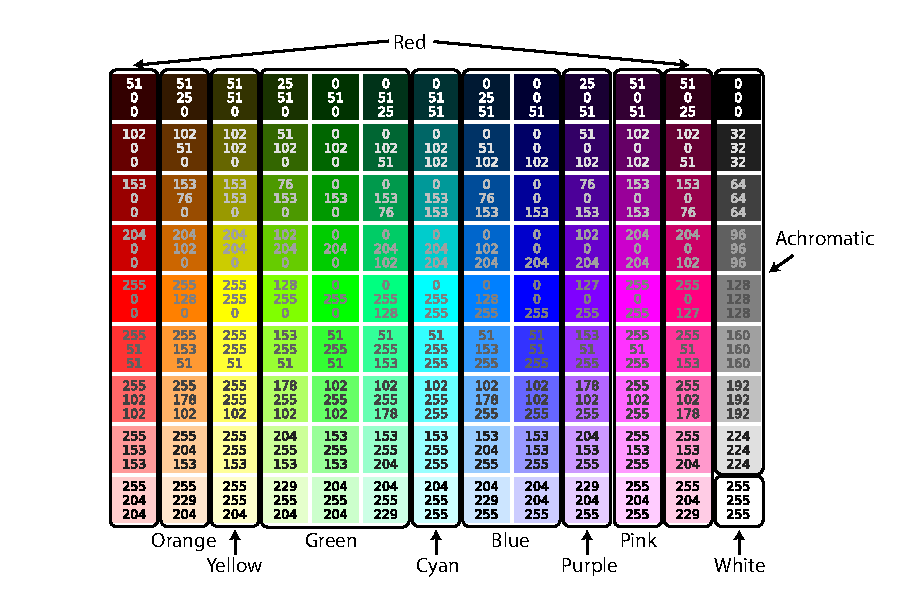
\includegraphics[width=0.5\textwidth]{figures/Col_tab.pdf}
	\caption{Set of 117 colours aggregated in 10 groups. For each colour, the three values represent the RGB components. \label{fig:colour_set}}
\end{figure}

Formally, let \(\vec{c_l} := \{ c^{\tt \scriptstyle R}_{l}, c^{\tt \scriptstyle G}_{l}, s^{\tt \scriptstyle B}_{l} \}\) with $l \in 1, ..., L$ denote each micro-colour. For each pixel \(\vec{s}_{ij}\) in an image, we find the micro-colour whose squared Euclidean dissimilarity with the pixel is minimal:
\begin{equation*}
c(\vec{s}_{ij}) := \operatornamewithlimits{argmin}_{l \in [1,L]} \| \vec{s}_{ij} - \vec{c}_{l} \|^{2}
\end{equation*}
The pixel is then associated with one out of $G = 10$ macro-colours, according to the groupings of micro-colours delineated in Figure~\ref{fig:colour_set}. This macro-colour, which we denote with $C(\vec{s}_{ij})$, is ultimately considered to be the pixel's colour.

For each colour $g\in 1, \dots, G$ we then define a binary matrix $B^{g} := (b_{ij}^{g})$, of the same dimensions as the considered drawing and whose components are 1 iff $g$ is the colour assigned to the pixel in question:~\footnote{Here and in the sequel, $\mathds{1}(A)$ denotes the \textit{indicator function} of event $A$, taking on the value 1 if $A$ is true, and 0 otherwise.}
\begin{equation}
	b_{ij}^{g} := \mathds{1}(C(\vec{s}_{ij}) = g)
\end{equation}
This enables us to define the \textit{pixel count} (i.e.~the number of pixels) of each colour $g$ in a given image as:
\begin{equation}
	n^{g} := \sum_{ij}b_{ij}^{g}
\end{equation}
Pixel counts can be used to compute the proportion of each colour in a given image or in a set of images, in order to answer the first type of research questions mentioned in section~\ref{introduction}. In section~\ref{sec:results_identification} below, we show the resulting proportions for the $N = 1212$ drawings of our sample, along with the decomposition into binary matrices of a couple drawings.

It is important to note that while the set of $L=117$ micro-colours used in this study is based on a typical RGB colour chart,~\footnote{such as the one available at \url{https://www.rapidtables.com/web/color/RGB_Color.html}} it could have been easily substituted with another one. The same holds for the set of $G$ macro-colours used here, which is the result of discussions in the ``Drawing of gods'' project team. Since it is complicated for computers and for human to differentiate black and grey (or which pencil was used by the children), they were grouped into a single ``achromatic'' category. Moreover, this distinction is not necessary to study a child's colour choice. Brown, which is considered as a colour of the second rank by \citet{pastoureau2017} and not as a hue in the Munsell system or in the HSV or HSL colour spaces for instance, is not included in the colour list. Indeed, brown is a shade of red or orange (eventually green) in these colour spaces, with a high saturation and a relatively low lightness or value. It would be possible to group some of the 117 micro-colours into a new ``brown'' group, however there was no consensus in the project team to decide which micro-colours should change macro-colour group.

\subsection{Quantification of colour diversity}
\label{sec:diversity}

There are a number of ways of quantifying the diversity associated with a discrete distribution, such as the distribution of colours in a drawing obtained with the identification method described in section~\ref{sec:identification} above. All diversity measures are, to a certain extent, dependent on the size of the sample from which the considered distribution has been obtained \cite[see e.g.][]{TweedieBaayen1998}, however the impact of this dependence is lessened in our case by the (partial) normalisation of drawing size (see section~\ref{sec:dataset_preprocessing} above). In the present study, we experiment with two diversity measures, namely the {\em variety} or number of distinct colours in a drawing, and the {\em Shannon entropy} of the colour distribution.

In the case of variety, an additional preprocessing step is performed: in order to reduce the amount of noise--anomalous pixels resulting from the digitisation process--a median filter of \(3 \times 3\) pixels is applied to each binary colour matrix $B^{g}$. The filtered matrix, $\tilde{B}^{g}$, is then used to compute new counts $\tilde{n}^{g} := \sum_{ij}\tilde{b}_{ij}^{g}$, which in turn make it possible to calculate the colour variety as:
\begin{equation}
	V := \sum_{g}\mathds{1}(\tilde{n}^{g} > 0)
\end{equation}

Following \citet{Shannon1948}, the colour entropy is defined as:
\begin{equation}
	H := -\sum_{g} f^{g}\mbox{ log }f^{g}
\end{equation}
where $f^{g}:= n^{g}/\sum_{k}n^{k}$ stands for the (unfiltered) colour relative frequency (computed on the basis of $B^{g}$). $H$ varies between 0 and log $G$: $H=0$ corresponds to a deterministic configuration where a single colour occurs with relative frequency $f^{g} = 1$, while the maximum $H=\mbox{log }G$ is reached when the colour distribution is uniform ($\forall g: f^{g} = 1/G$).

{\color{green}[AX: comme de fait on ne repond pas a la question "relation age -- diversite des couleurs", je modifierai ci-dessous pour y referer moins directement (apres avoir fini avec la section 4.2)]}
In section~\ref{sec:results_diversity} below, we will show how these two ways of quantifying colour diversity make it possible  permit to answer SSH research questions, such as the last one mentioned in section~\ref{sec:introduction} about the number of colours used in a subset of drawings according to the age of children (or to another feature). Moreover, as illustrated in the section~\ref{sec:results_entropy_variety}, it is also possible to detect children's strategies in the task of drawing god, also a goal of the psychologists of the project team. {\color{red} [Tentative de transition, est-ce que ca vous convient?]}

\section{Results}
\label{sec:results}

In this section, we present the first results obtained by applying the methods for colour identification and colour diversity assessment described in section~\ref{methods} to the selected subset of the ``Drawings of gods'' database.
%Here, we first show an explicit sample of the results obtained from the method Identification of colours (see section \ref{sec:identification}) applied on all drawings. 
%We then extend the presentation of these results using the method of Colour diversity retrieval (see section \ref{sec:diversity}) crossed with the results of a deeper measure of variety commonly used in Computer Vision. 
%The first step of the colour experiment depicted in section \ref{sec:set_col_definition} is presented in order to asses the automatic method of variety estimation in face of human perceived variety.

\subsection{Colour identification}
\label{sec:results_identification}

The first outcome of the proposed colour identification method is the decomposition of each image into a set of $G$ binary matrices, one matrix $B^g := (b_{ij})$ per colour $g$. One way of visualising these matrices consists in using them as an inverted ``mask'', in the sense of image processing, and applying them to the original image. Formally, for each colour $g$, we construct a new image $S^g := (\vec{s}^{\,g}_{ij})$, where each pixel is defined as:
\begin{equation}
	\vec{s}^{\,g}_{ij} := 
	\begin{cases} 
		\vec{s}_{ij} \mbox{ if } b^g_{ij} = 1 \\
		(0, 0, 0) \mbox{ otherwise} 
	\end{cases}
\end{equation}
The result is a set of $G$ images filled with black except for the pixels that have been identified as belonging to a given colour $g$. Figure~\ref{fig:example} below shows three examples of this way of visualising the colour configuration detected in an image.

\begin{figure*}
	\centering
	$\vcenter{\hbox{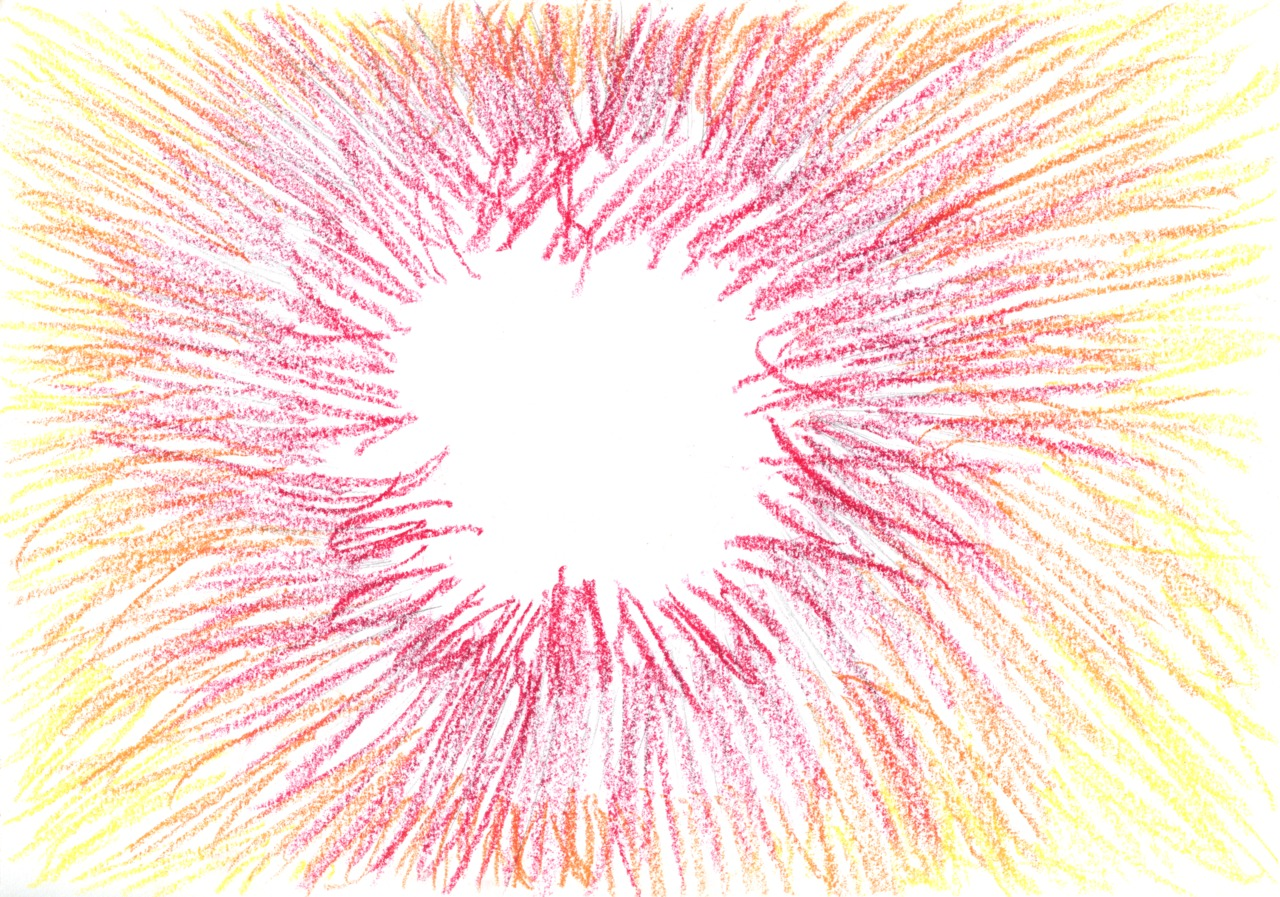
\includegraphics[width=0.37\linewidth]{figures/jp04_ko_m_ryx_13_09_kmx-r.jpg}}}$
	$\vcenter{\hbox{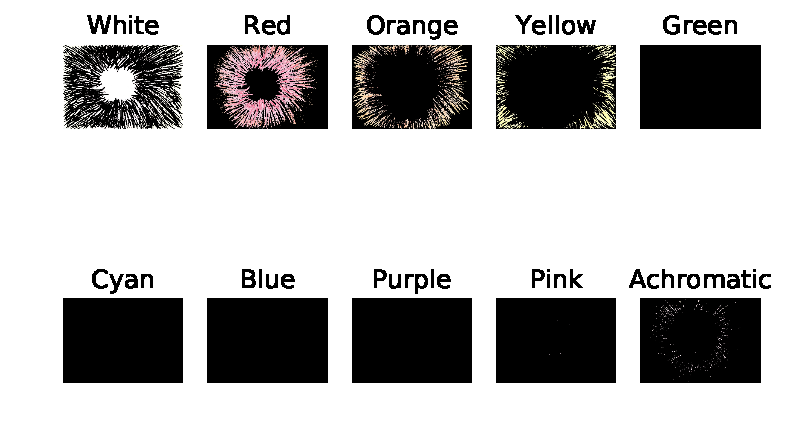
\includegraphics[width=0.62\linewidth]{figures/jp04_ko_m_ryx_13_09_kmx-rno_filter_mask.pdf}}}$\hfil
	\vspace{0.075\textheight}
	$\vcenter{\hbox{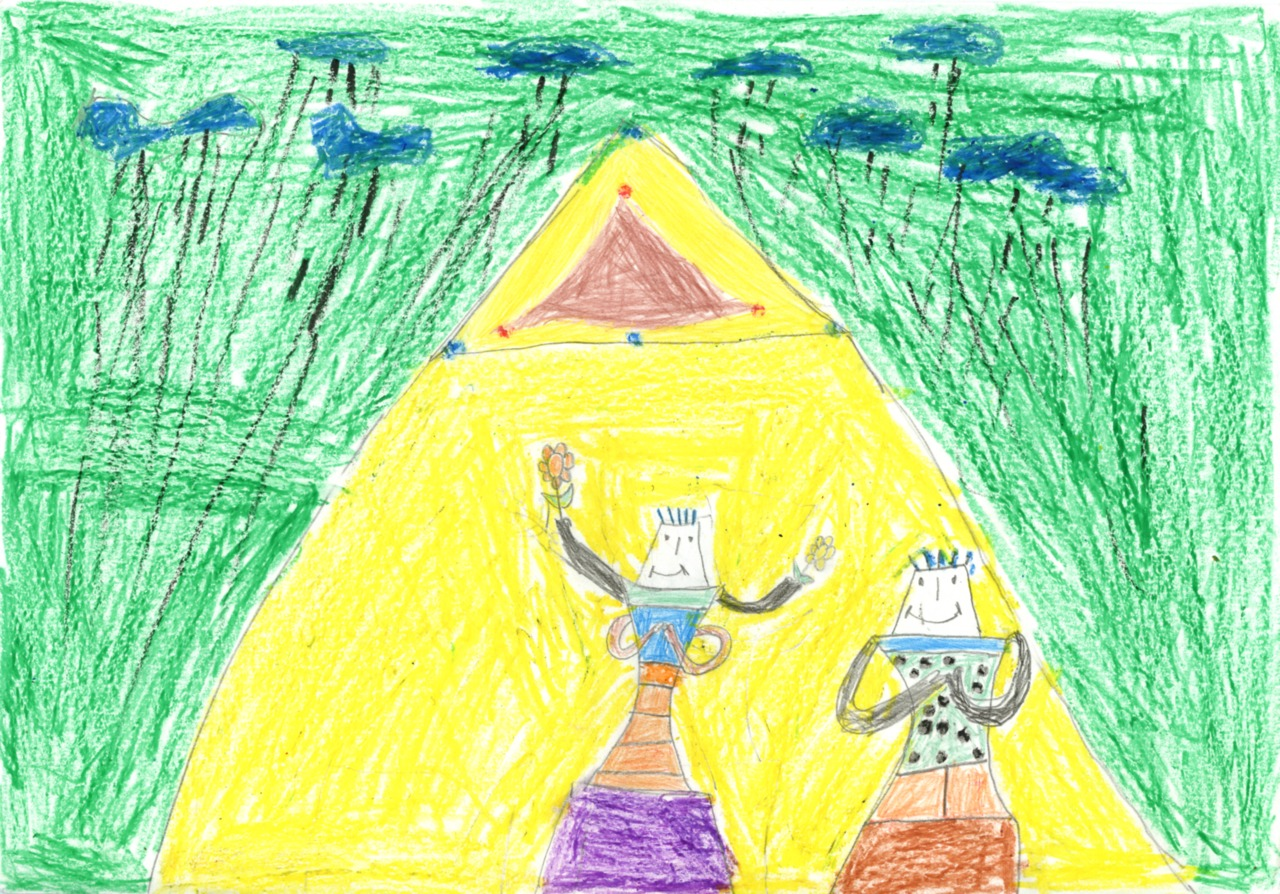
\includegraphics[width=0.37\linewidth]{figures/ru08_bo_f_pb_07_05_ali-r.jpg}}}$
	$\vcenter{\hbox{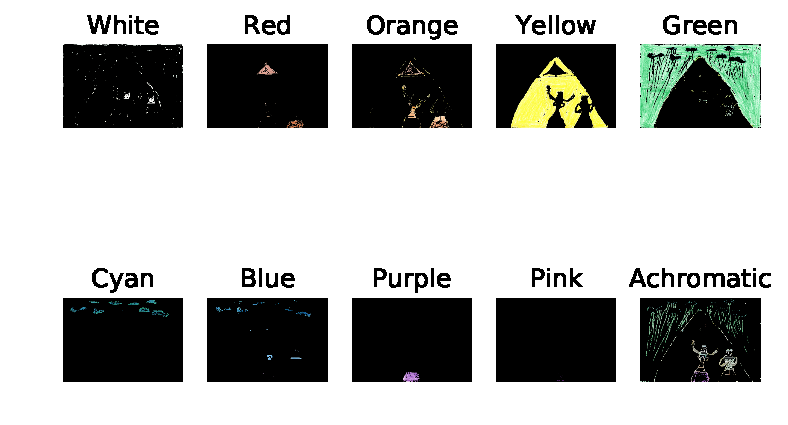
\includegraphics[width=0.62\linewidth]{figures/ru08_bo_f_pb_07_05_ali-rno_filter_mask.pdf}}}$\hfil
	\vspace{0.075\textheight}
	$\vcenter{\hbox{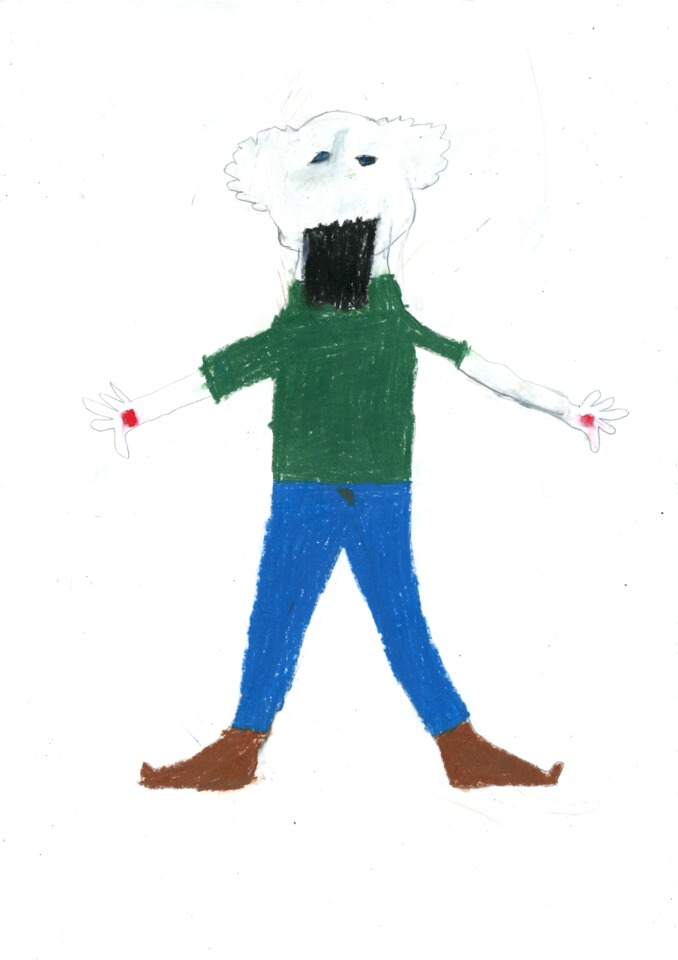
\includegraphics[width=0.32\linewidth]{figures/ch16_fr_m_rec_13_07_rap-r.jpg}}}$\hspace{0.038\textwidth}
	$\vcenter{\hbox{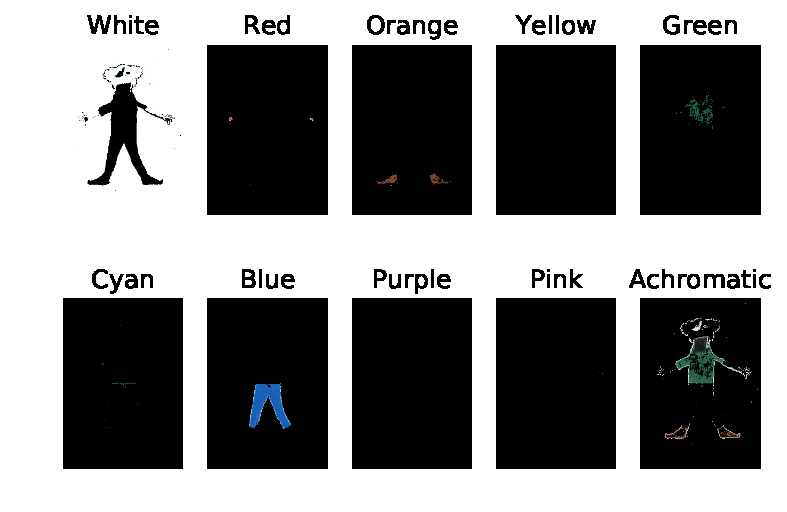
\includegraphics[width=0.62\linewidth]{figures/ch16_fr_m_rec_13_07_rap-rno_filter_mask.pdf}}}$
	\caption{Visualising the results of the colour identification method. Top: Japanese drawing. Middle: Russian drawing. Down: Swiss drawing.}
	\label{fig:example}
\end{figure*}

These examples were selected to illustrate various (and decreasing) degrees of concordance between the automated colour identification and the human intuition. In the first example, all colours are identified as expected by the project's team, which is what visual inspection of the results generally reveals. All colours are also identified correctly and as expected in the second example, considering that brown is not part of the selected colour set; as a result it is divided into orange and red. Also, and it is coherent, the mixing of blue and yellow around the centre of the drawing creates nuances that are identified as green. The third example illustrates a weakness of the method, namely the identification of highly saturated colours, in particular green.
%first example illustrates a good extraction of the main colours whereas the second illustrates a less good colour extraction because of the similar computed distances between $\vec{s}$  pixel and the two or more $G$ main colours e.g.~$g = \mbox{Green}$ and $g = \mbox{Achromatic}$. 
%Also, the lack of the main colour Brown in the defined set of colours produces errors during the colour identification process as well as a over attribution of the pixels to the Green when yellow and grey overlap into the drawing. Except these problems with low saturated colours, an other typical problem occurs when two colours are mixed, such as grey and yellow which are detected as green. This type of mixing represents only a few pixels in a drawing and thus, does not affect percentages of colours. However, for this reason, $B^g$ is transformed into $\tilde{B}^g$ to count the number of pixels. Despite these errors, the results are good enough for the majority of drawings. As it was not possible to create a gold standard, the quality was assessed visually.

%{\color{red}[CC: Other distances tested, such the one from Androutsos 1999 et un autre plus récent et mieux, add ref in 4.1 for fig. 3]}

%{\small \color{teal}[IDEE: Cross validation en prennant al\' eatoirement quelques pixels par dessin et les attribuer manuelle \`a une couleurs principales ou avoir un toy example avec un dessin o\`u l'on "connait" les couleurs.]}

Besides the visualisation of colour decomposition, the method allows us to compute the proportion of each colour $g$ in the selected dataset, based on the summation of each colour's pixel counts (with the exception of white) over all drawings. The resulting histogram, represented in Figure~\ref{fig:propcolours} shows that the most frequently identified ``colour'' is achromatic, followed by blue and yellow. Orange, red, green and cyan have a moderate representation, while pink and purple are clearly underrepresented. Studies on colour preference \cite[see e.g.][]{Granger1955,Zentner2001,JonauskaiteMohrAntoniettiEtAl2016} have shown that shades of blue and green, such as cyan, as well as red (especially for female and 3- to 4-year old children) are the most preferred colours, while the least preferred ones are yellow and orange (and sometimes red). The distribution of identified colours in our data shows that children certainly do not use their preferred colours to draw god, but specific colours for this task. Assuming that they employ blue to depict the sky and yellow for the light or the sun, the results are compatible with the hypothesis that children imagine god as something or someone shining in the sky. The proposed method will also make it possible to compare the colour distribution across countries, age groups, and so on, and thus to test various psychological hypotheses.

\begin{figure}[h!]
	\centering
	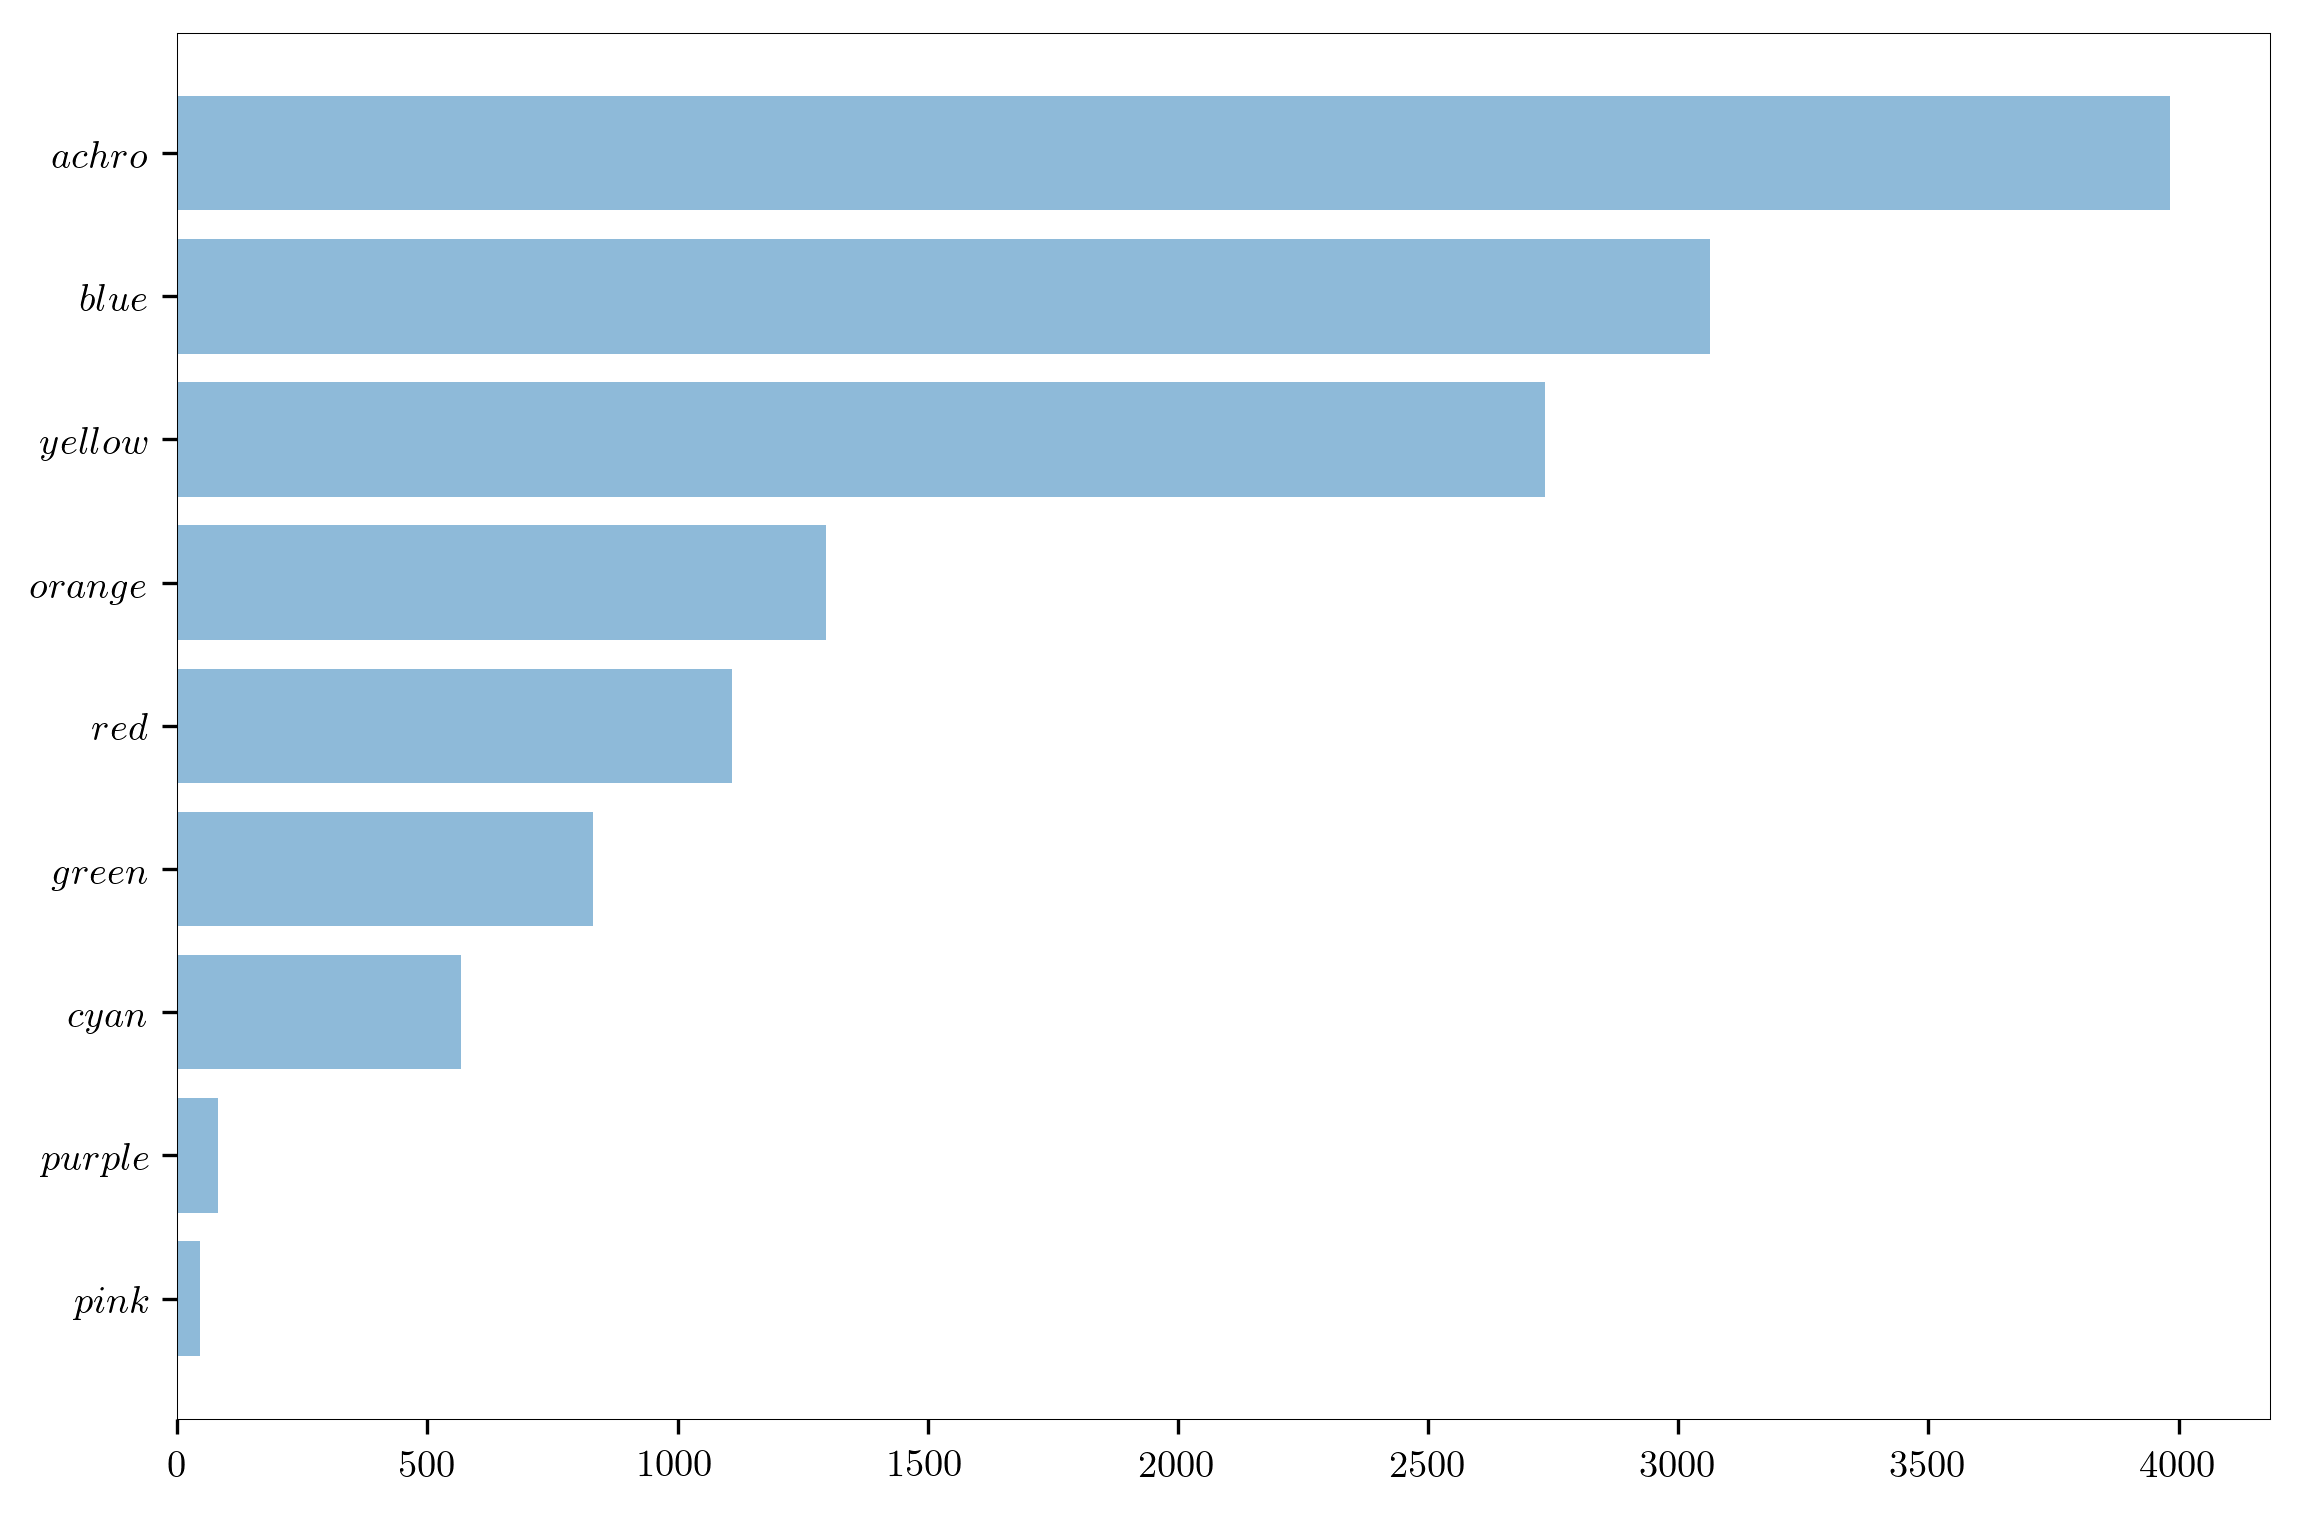
\includegraphics[width=\linewidth]{figures/colors-barplot.png}
	\caption{Distribution of identified colours.}
	\label{fig:propcolours}
\end{figure}

\subsection{Quantification of colour diversity}
\label{sec:results_diversity}

\subsubsection{Variety and entropy}
\label{sec:results_entropy_variety}

Based on the output of the colour identification method, the variety and entropy of colours were computed as described in section~\ref{sec:diversity}. Figure~\ref{fig:variety_histogram} shows the distribution of colour variety in the dataset, which reveals that a majority of drawings (about 70\%) have between 5 and 8 identified colours. The distribution deviates slightly from normality, in the sense that drawings with 7 and 8 colours are particularily frequent, and there is also a small peak of drawings with a single non-white colour ($V=2$). The box-plots in Figure~\ref{fig:entropy_boxplot} depict the variability of colour entropy for a given amount of  colour variety. While the median of entropy is consistently increasing with variety, as expected, the spread of individual entropy values is quite large regardless of the corresponding variety.
 
\begin{figure}[h!]
	\centering
	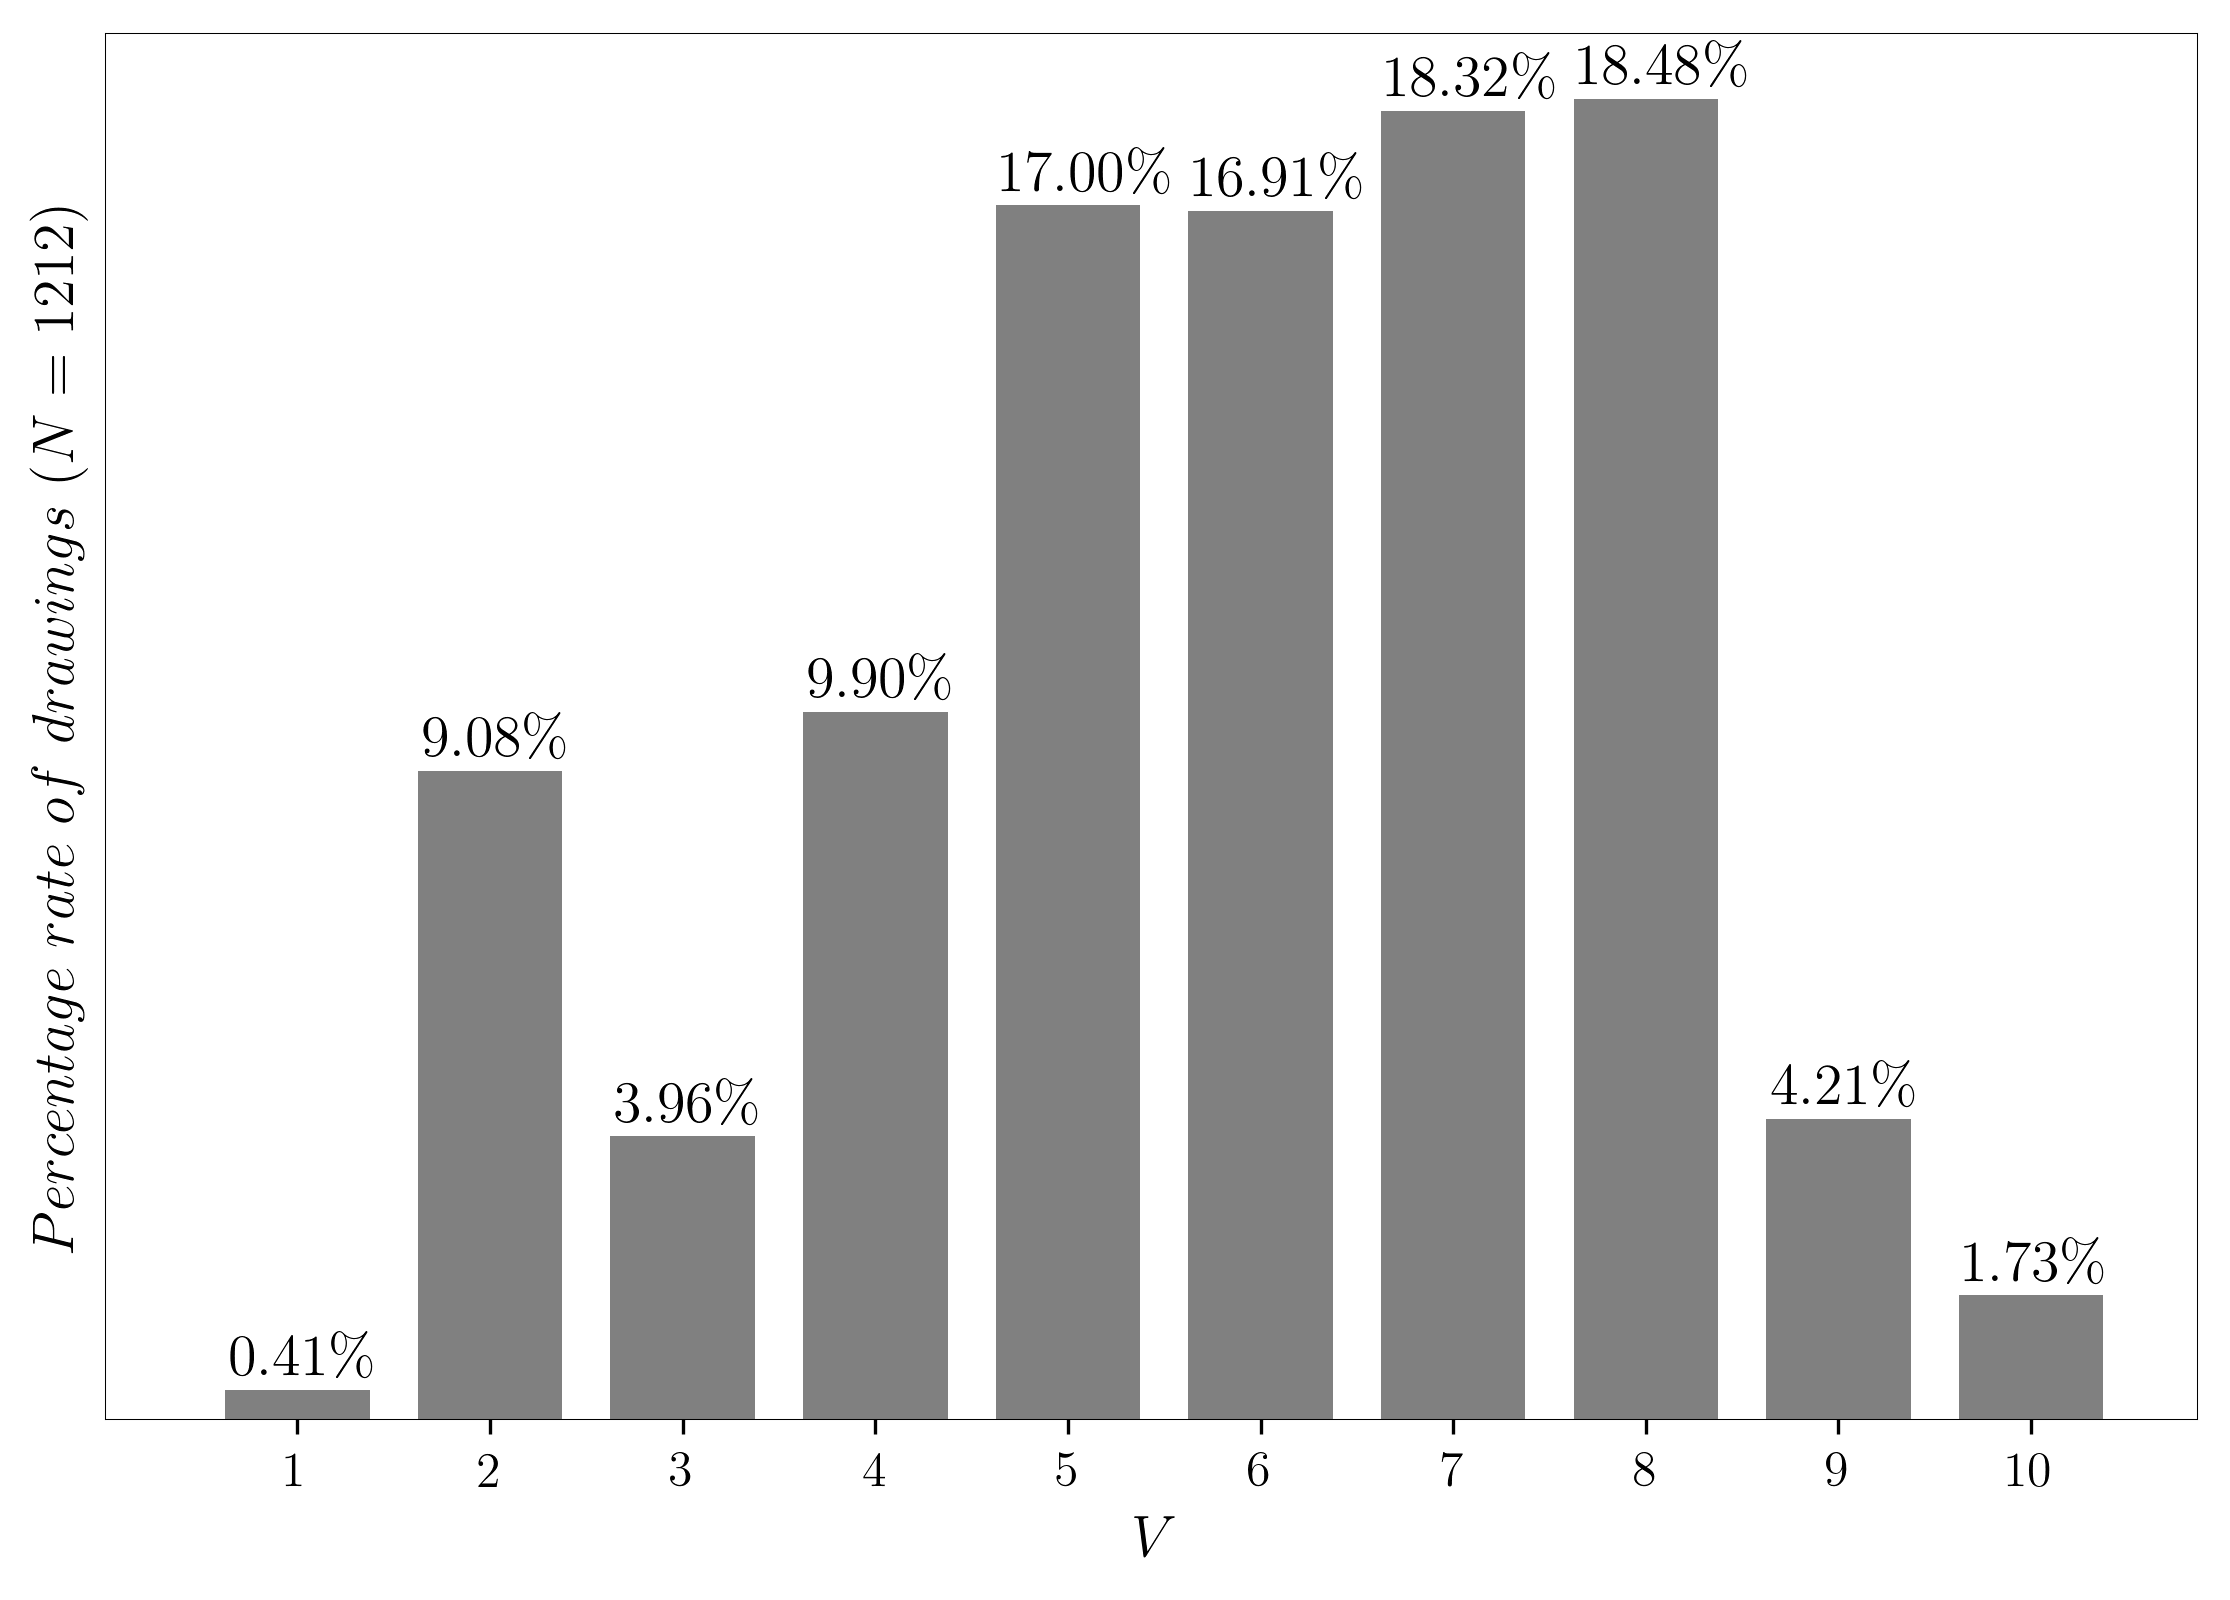
\includegraphics[width=\linewidth]{figures/colors-boxplot-hist.png}
	\caption{Distribution of colour variety}
	\label{fig:variety_histogram}
\end{figure}

\begin{figure}[h!]
	\centering
	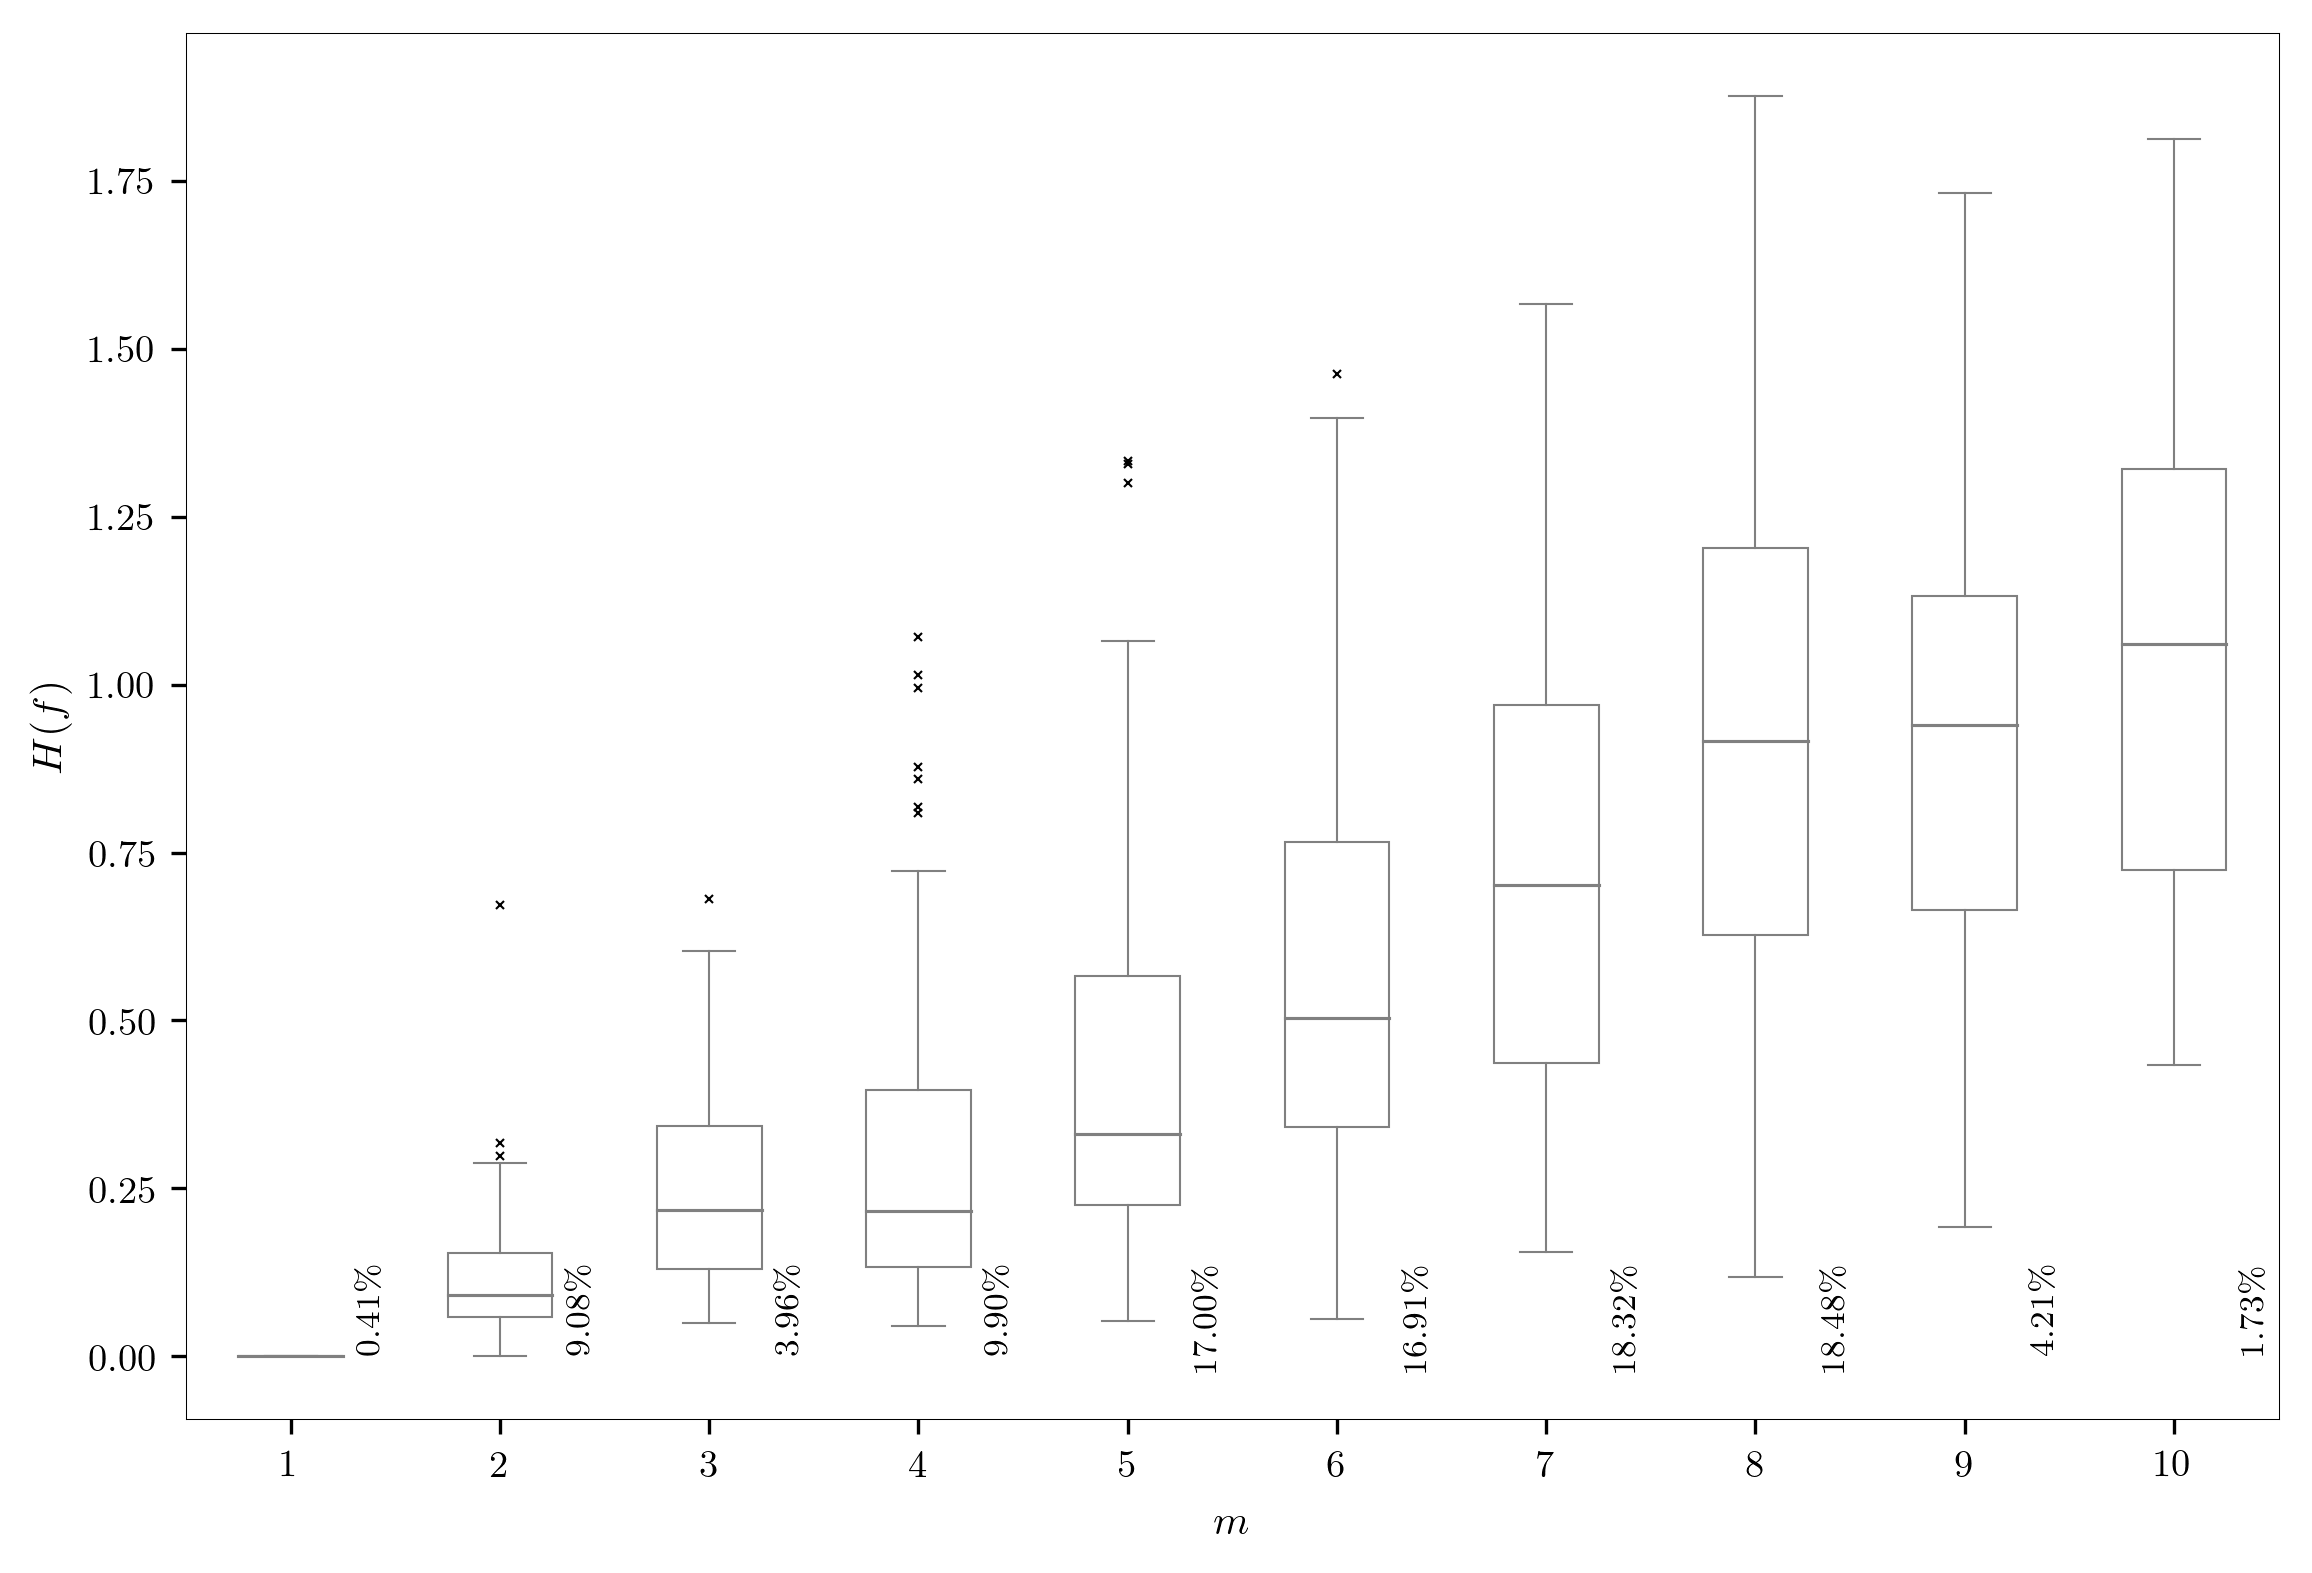
\includegraphics[width=\linewidth]{figures/colors-boxplot.png}
	\caption{Colour entropy box-plots as a function of colour variety.}
	\label{fig:entropy_boxplot}
\end{figure}

In order to get a better idea of the interpretation of colour entropy variations for a given amount of variety, we have designed a visualisation in which a sample of drawings are plotted on a grid with 9 rows corresponding to colour variety (between 2 and 10, excluding empty drawings) and 5 columns corresponding to specific points in the distribution of colour entropy (minimum, first quartile, median, third quartile, and maximum), as represented in Figure~\ref{fig:grille}. In practice, this visualisation was constructed one row after another, by extracting all drawings with a given amount of colour variety in the dataset, then finding in this subset the drawings with the minimum and maximum colour entropy as well as those that are closest to the desired quantiles. This representation shows that colour entropy seems to correspond well with the intuitive notion of drawing completeness: the higher the entropy, the more the colours are covering the page. Also, entropy and variety seem to concur to create a gradual distinction between drawings with a white background and single object (bottom-left) and drawings representing one or more objects in a more contextualized fashion (top-right). Thus, besides operationalizing the basic notion of colour diversity, colour variety and entropy enable us to characterize certain aspects of drawing ``strategy'' and of the spatial organisation of colours in a drawing.

\begin{figure*}
	\centering
	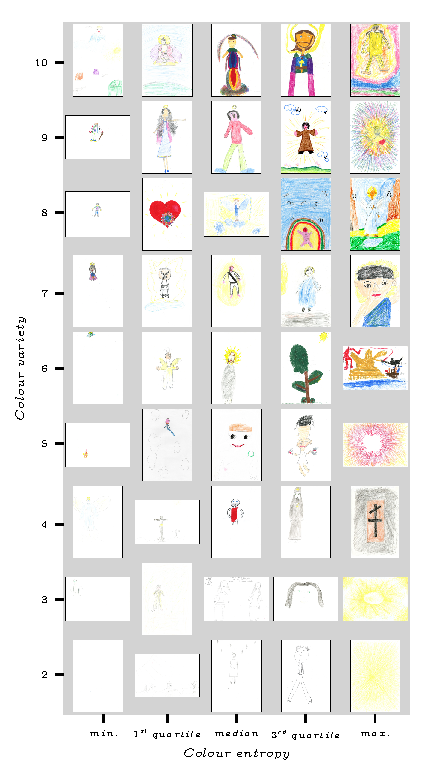
\includegraphics[width=0.75\linewidth]{figures/colors-grille.pdf}
	\caption{Sample of drawings illustrating selected points in the distribution of colour entropy (columns) as a funtion of colour variety (rows).}
	\label{fig:grille}
\end{figure*}

{\color{green}[AX: je m'arrete ici pour le moment.]}

Based on the chosen colour sets, the entropy measure is sensitive to the errors during the pixel colour attributions (e.g.~similar distances, no Brown, etc.). 
Then, we compare it with a common approach of Computer Vision which consists to measure the entropy on the greyscale levels histogram of the drawing. 
The scatter plot, figure~\ref{fig:entropies}, depicts the significant Pearson correlation ($r=0.8866$, $p=0.000$) between these two entropy values. % {\color{red}[Reprendre quelques parties de 3.5 et citer \citet{wu2013}]}. 

%{\small \color{teal}[IDEE: Est-ce que les extr\`emes ne permettraient pas d'en dire plus? A creuser.]}

\begin{figure}[h!]
	\centering
	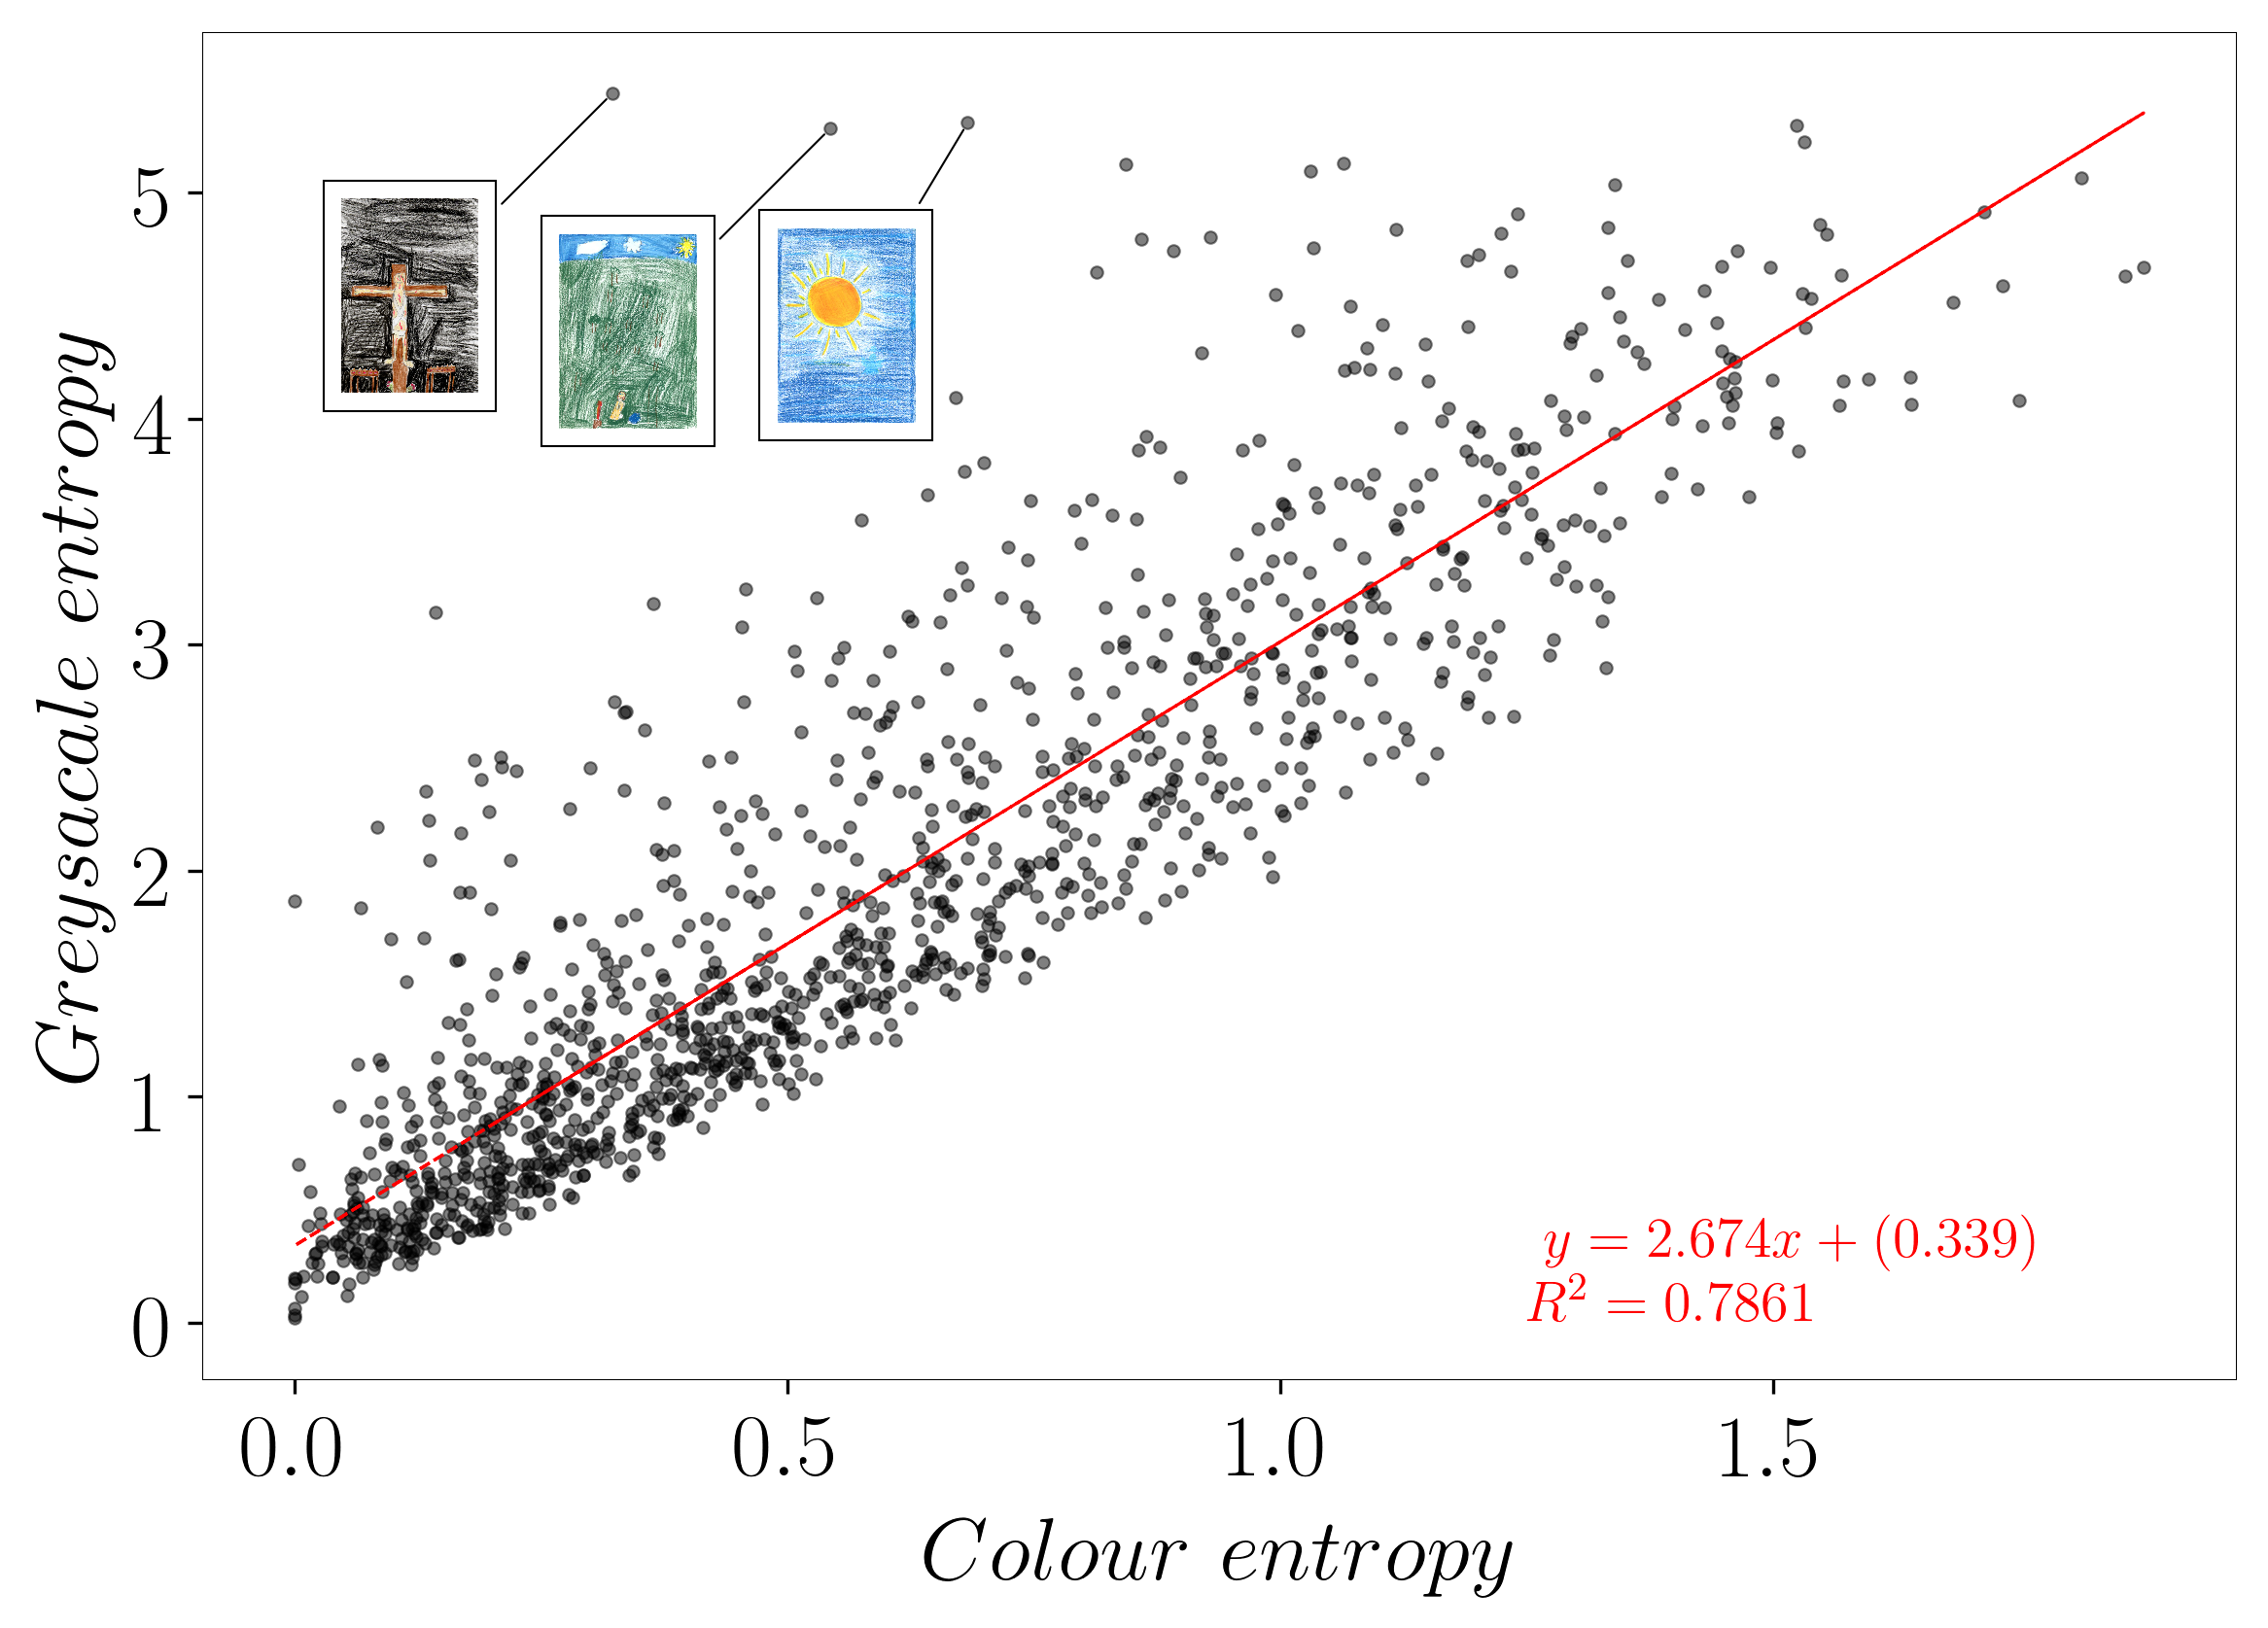
\includegraphics[width=\linewidth]{figures/colors-greysacale-entropies.png}
	\caption{Scatter plot of the entropies on the greyscale levels histogram with the main colours entropies.}
	\label{fig:entropies}
\end{figure}

\subsubsection{Variety concordance} {\color{red} Titre a modifier}
\label{sec:results_variety_concordance}

For each $\tilde{k}$ drawing in a sample of $\tilde{N} = 10$ drawings, we evaluate the concordance of the variety computed automatically $v^c_i = {1, \dots, G}$, by the algorithm of section \ref{sec:identification} {\color{red} Plutot selon $V$ de la section 4.5}, and the human perceived variety $v^h_i = {1, \dots, +\infty}$. 

{\color{red}[CC: a modifier, juste pour montrer que c'est autre chose que l'autre partie de l'experience]}
More precisely, we asked five human experts (the same ones as described in the section~\ref{sec:set_col_definition}) to write all the colours they saw in each drawing.
The annotators had at their disposal 15 spaces to write the colour names.
Only two annotators considered "white" as a colour of the drawing and thus it was removed from the results.
To count the number of colours found by each annotator, we counted the number of spaces filled. 
For instance, if an annotator wrote several colour or shade names in a same space to describe one colour, it was counted as one colour.


First, we observe on Figure~\ref{fig:compnbcolourssd} that the numbers of colours identified automatically is different to the humans in a range of two colours in average. 
These results are quite impressive in face of the number of factors considered during both estimations of variety; on one hand the errors of the automatic attributions observed previously and, on the other hand, the human perception bias. 
The Figure \ref{fig:compnbcoloursscatter} confirms this trend with a linear relationship.

\begin{figure}[h!]
	\centering
	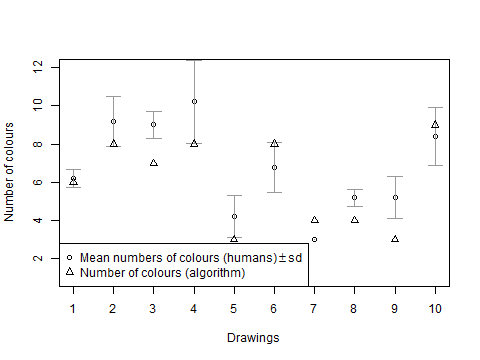
\includegraphics[width=\linewidth]{figures/comp_nb_colours_sd.png}
	\caption{Drawings in function of the means numbers of colours estimated by the algorithm and human.}
	\label{fig:compnbcolourssd}
\end{figure}

\begin{figure}[h!]
	\centering
	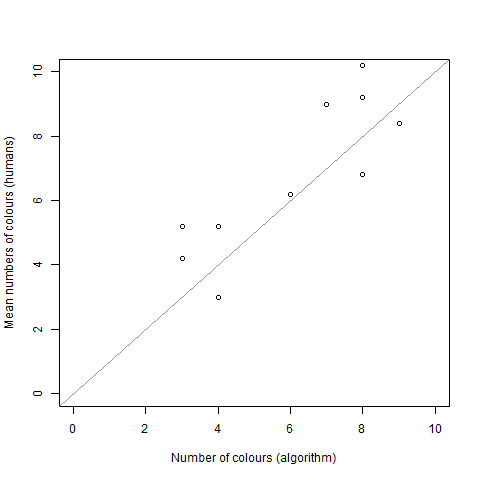
\includegraphics[width=\linewidth]{figures/comp_nb_colours_scatter.png}
	\caption{Scatter plot of the variety observed by human in function of the automatic estimation of the variety.}
	\label{fig:compnbcoloursscatter}
\end{figure}



The Figure~\ref{fig:blandandaltman} shows the range of the disagreement using the \textit{Bland and Altman graphic} \cite{bland1986}.
The differences between the varieties of each $i$ drawing,  $d_i = v^c_i - v^h_i$, are represented in function of their means $\overline{d}_i = v^c_i + v^h_i/2$. 
The range of disagreement $d_i$ is then analysed in function of the mean $\overline{d}_i$. More $d_i$ is distant of  $0$, respectively close, $d_i \rightarrow 0$ , more the disagreement is higher, respectively concordant,  whereas $\overline{d} = 1/N\sum_{i}^{\tilde{N}}d_i = 0$ depicts a perfect concordance between these two varieties. 



Although there is no significant disagreement under the normal distribution hypothesis, the low size $\tilde{N}$ of the sample is not representative and show a mean disagreement $\overline{d}=-0.74$ {\color{red}[AJOUTER LA VALEUR DE D\'ESACCORD, CC: FAIT MAIS ETRE MOINS NEGATIF, deja un essai et explication]}. It is coherent that there are more colours found by humans than by the algorithm, since the brown is not detected automatically and the grey and the black were aggregated.


\begin{figure}[h!]
	\centering
	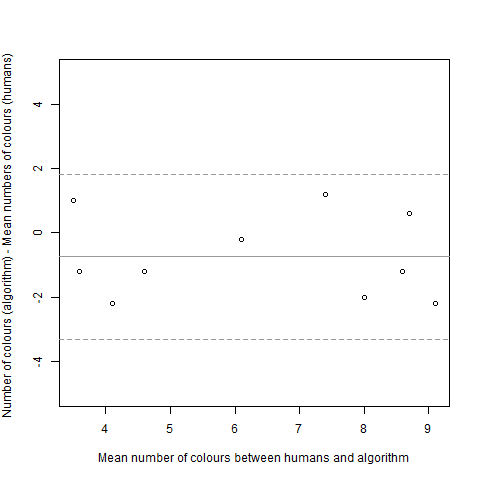
\includegraphics[width=\linewidth]{figures/comp_nb_colours_agreement.png}
	\caption{Range of disagreement of variety estimations using Bland et Altman  Graphic.}
	\label{fig:blandandaltman}
\end{figure}



\section{Conclusion}
\label{sec:conclusion}
In this paper, we have proposed a simple and efficient method to identify colours in children's drawings (and in other type of images), adapted to answer SSH research questions, as well as two ways of quantifying colour diversity based on the results of colour identification.
The methods were tested on a subset of data of the project ``Drawings of gods'' in this paper and will be employed systematically in the future in the project to answer various research questions based on various features related to children, such as their age, their country or their gender. Unlike usual inter-ratter methodology in psychology which ask to a few humans to annotate the data, a task which is exhausting and difficult with a large number of these complex drawings, the methods exposed in this paper have the advantage to be objective and constant on a large volume of data. 
Moreover, as illustrated in the section~\ref{sec:results_entropy_variety}, the methods allow us to go further in answering the project research questions. Indeed, a set of children's strategies to draw god can be detected, such as filling the complete page or drawing only a main character or object without background.

The proposed method of colour identification also introduces the advantage to be adaptable, as explained in the section~\ref{sec:identification}, since the set of micro- and macro-colours can be easily modified for specific SSH research purposes. For instance, as suggested in the section~\ref{sec:state_of_the_art}, one of these colour sets could be replaced by the ones defined with colour-naming methods.

While the methods were illustrated on data extracted from the project ``Drawings of gods'', they are easily applicable to other SSH  research dataset. For instance, it would be possible studying the main colours used by a painter according to various periods of his/her life; or comparing the mean number of colours of cover pages of a magazine in the various seasons of a year.

As a next step, it could be interesting to apply a filter at the beginning of the process, such as the Mumford-Shah regularizer proposed by \citet{erdem2009} which transforms a set of noisy pixels in an uniform patch. 
Indeed, when children (or adults) fill in an area of the sheet with one colour, the application is not regular and consequently not all pixels of the zone are coloured. 
Thus, in order to avoid underestimating the proportion of one particular colour, standardizing colours by zone could help work around the possible issue.


\bibliography{bibliography}
\bibliographystyle{acl_natbib}

\end{document}
